\documentclass[twocolumn,aps,prl]{revtex4-1} % For final two-column format
%\documentclass[twocolumn,aps,prl]{revtex4-1} % For double-spaced, single-column draft
\usepackage[utf8]{inputenc}
%%% Sample LaTeX file for Physics 107
%%% I (M.S.-S.) typically edit in TeXworks and use pdfLaTeX as the typesetting engine
\usepackage{graphicx}% Include figure files
\usepackage{amsmath,amssymb}
\usepackage{gensymb}

\usepackage{comment}


% It may be convenient to define shortcut commands such as these:
\newcommand{\ket}[1]{\ensuremath{\vert #1 \rangle}}
\newcommand{\abs}[1]{\ensuremath{\vert #1 \vert}}
\renewcommand{\vec}[1]{\ensuremath{\mathbf{#1}}}
\newcommand{\uvec}[1]{\ensuremath{\hat{\vec{#1}}}}

\begin{document}

\title{Behavior of Flux Vortices in Superconducting Niobium}

\author{Kevin Chaves, Litawn Gan, Leonard Lupin-Jimenez, Mason Rogers}
\affiliation{Department of Physics, Stanford University, Stanford, California 94305, USA}


\begin{abstract}
We use Hall sensor measurements to understand the behavior of vortices in superconducting Niobium. With a Hall sensor of side length $1$mm, we observe two interesting macroscopic patterns in vortex behavior. The first yields a measurement of the upper critical field $H_{c2}$ for the sample of $427(5)$mT and 424(9) mT using different estimation methods. The second corresponds to an eviction of vortices upon reducing field below a critical threshold of $100.84(14)$mT. We discuss avenues for further experimentation, including more precise observation techniques to analyze smaller-scale behavior and explanations for the redistribution of vortices beneath our measured threshold.
\end{abstract}
\maketitle

%Intro
In a phenomenon known as the Meissner Effect, superconductors placed in small external magnetic fields admit no magnetic flux through their interiors. As the external magnetic field increases, this effect breaks down in one of two ways. In type I superconductors, there is one critical value of external field above which the superconductor is forced into a normal state, permitting flux uniformly. In type II superconductors, there are two critical field strengths. Below the lower critical field $H_{C1}$, no flux is permitted, and above the upper critical field $H_{c2}$, flux is permitted uniformly. The distinguishing region lies between $H_{c1}$ and $H_{c2}$, within which the superconductor admits flux in quantized packages known as vortices. Each vortex carries one flux quantum, or $2.067(10)^{-15}$Wb, with a width dependent on the coherence length $\xi$ and penetration depth $\lambda$ of the superconductor in question. In the case of pure niobium, one of the three elemental type II superconductors and the focus of this paper, we have $\xi = 38$nm and $\lambda = 47$nm. Accordingly, the width of vortices of niobium is of that scale.

Because of their small size, observing individual vortices is a difficult challenge. Recently, there has been success in imaging vortices with small ($\sim 0.5\mu$m) Hall sensors and scanning SQUIDs; however, aggregate properties of vortices are still poorly understood. \cite{SQUID} The statistical behavior of vortices depends on many factors. In principle, vortices are mobile, moving at speeds limited primarily by an effective viscosity in the superconductor. \cite{VortexMotion_1} In practice, imperfections in the superconductor itself yield a nonuniform potential energy landscape for the vortices, causing them to `pin' to locally energy-minimizing configurations. Moreover, freely-moving vortices experience long range mutual repulsion from each other as a result of a small current circulating each flux line, resulting in complex macroscopic arrangement phenomena. \cite{VortexInteraction_1} A final phenomenon of interest is that of flux trapping. If the magnetic field is reduced, vortices can potentially remain trapped in the superconductor, implying that their statistical behavior depends on the highest field to which the superconductor has been exposed while superconducting. These deviations from ideal behavior beg questions about macroscopic behaviors of vortex fields. We aim to use Hall sensor measurements to understand constraints on vortex motion, vortex positioning, and flux trapping as they pertain to the bulk behavior of flux lines emitted by large groups of vortices.

%Methods

Hall sensors exploit the Hall effect to measure magnetic field, whereby the deflections of charge carriers moving through a magnetic field result in a potential gradient transverse to both the current and the field. In a uniform field, the Hall voltage responds linearly both to the applied current and the strength of the applied field. We aim to see how this response differs in the presence of a vortex field, which is inherently nonuniform. In order to observe individual vortex motion, each cross section of a Hall cross must be on the order of single vortex. 

Two sets of Hall cross designs were fabricated for the experiment. Each device would have four Hall crosses covered by bulk niobium and two Hall crosses not covered by the niobium for control. One set of devices had cross sectional lengths of 5$\mu$m while the other set had cross sectional lengths of 900nm. The 5$\mu$m Hall crosses were designed to measure the shape of the distribution of the number of flux quanta in the Hall bar sensitive region at any particular applied field strength. The 900nm Hall crosses were designed to detect single vortices without the use of e-beam lithography. This would indicate the quantity of vortices in the detection region, allowing us to look at spatial and temporal variations in vortex populations.

To determine reasonable experimental parameters, we simulated the deflection of electrons in a field of non-interacting vortices. The simulation indicated that for low densities of vortices, the spatial configuration of vortices had a significant impact on the measured voltage. For uniformly spaced vortices, Hall voltages approached that of an equal flux of uniform density; for clustered vortices, Hall voltages approached zero. However, once the number of vortices in the sensitive region reached 30, the variation in voltage response had diminished significantly, and measured voltages became nearly indistinguishable from the corresponding voltages due to a uniform field. Furthermore, the voltage response scaled linearly with current up to $\sim$50$\mu$A, at which point the Hall effect tapered off due to the finite supply of electrons. At currents as small as 100nA, the effect was still palpable; hence, we settled on a current of 250nA.

\begin{figure}
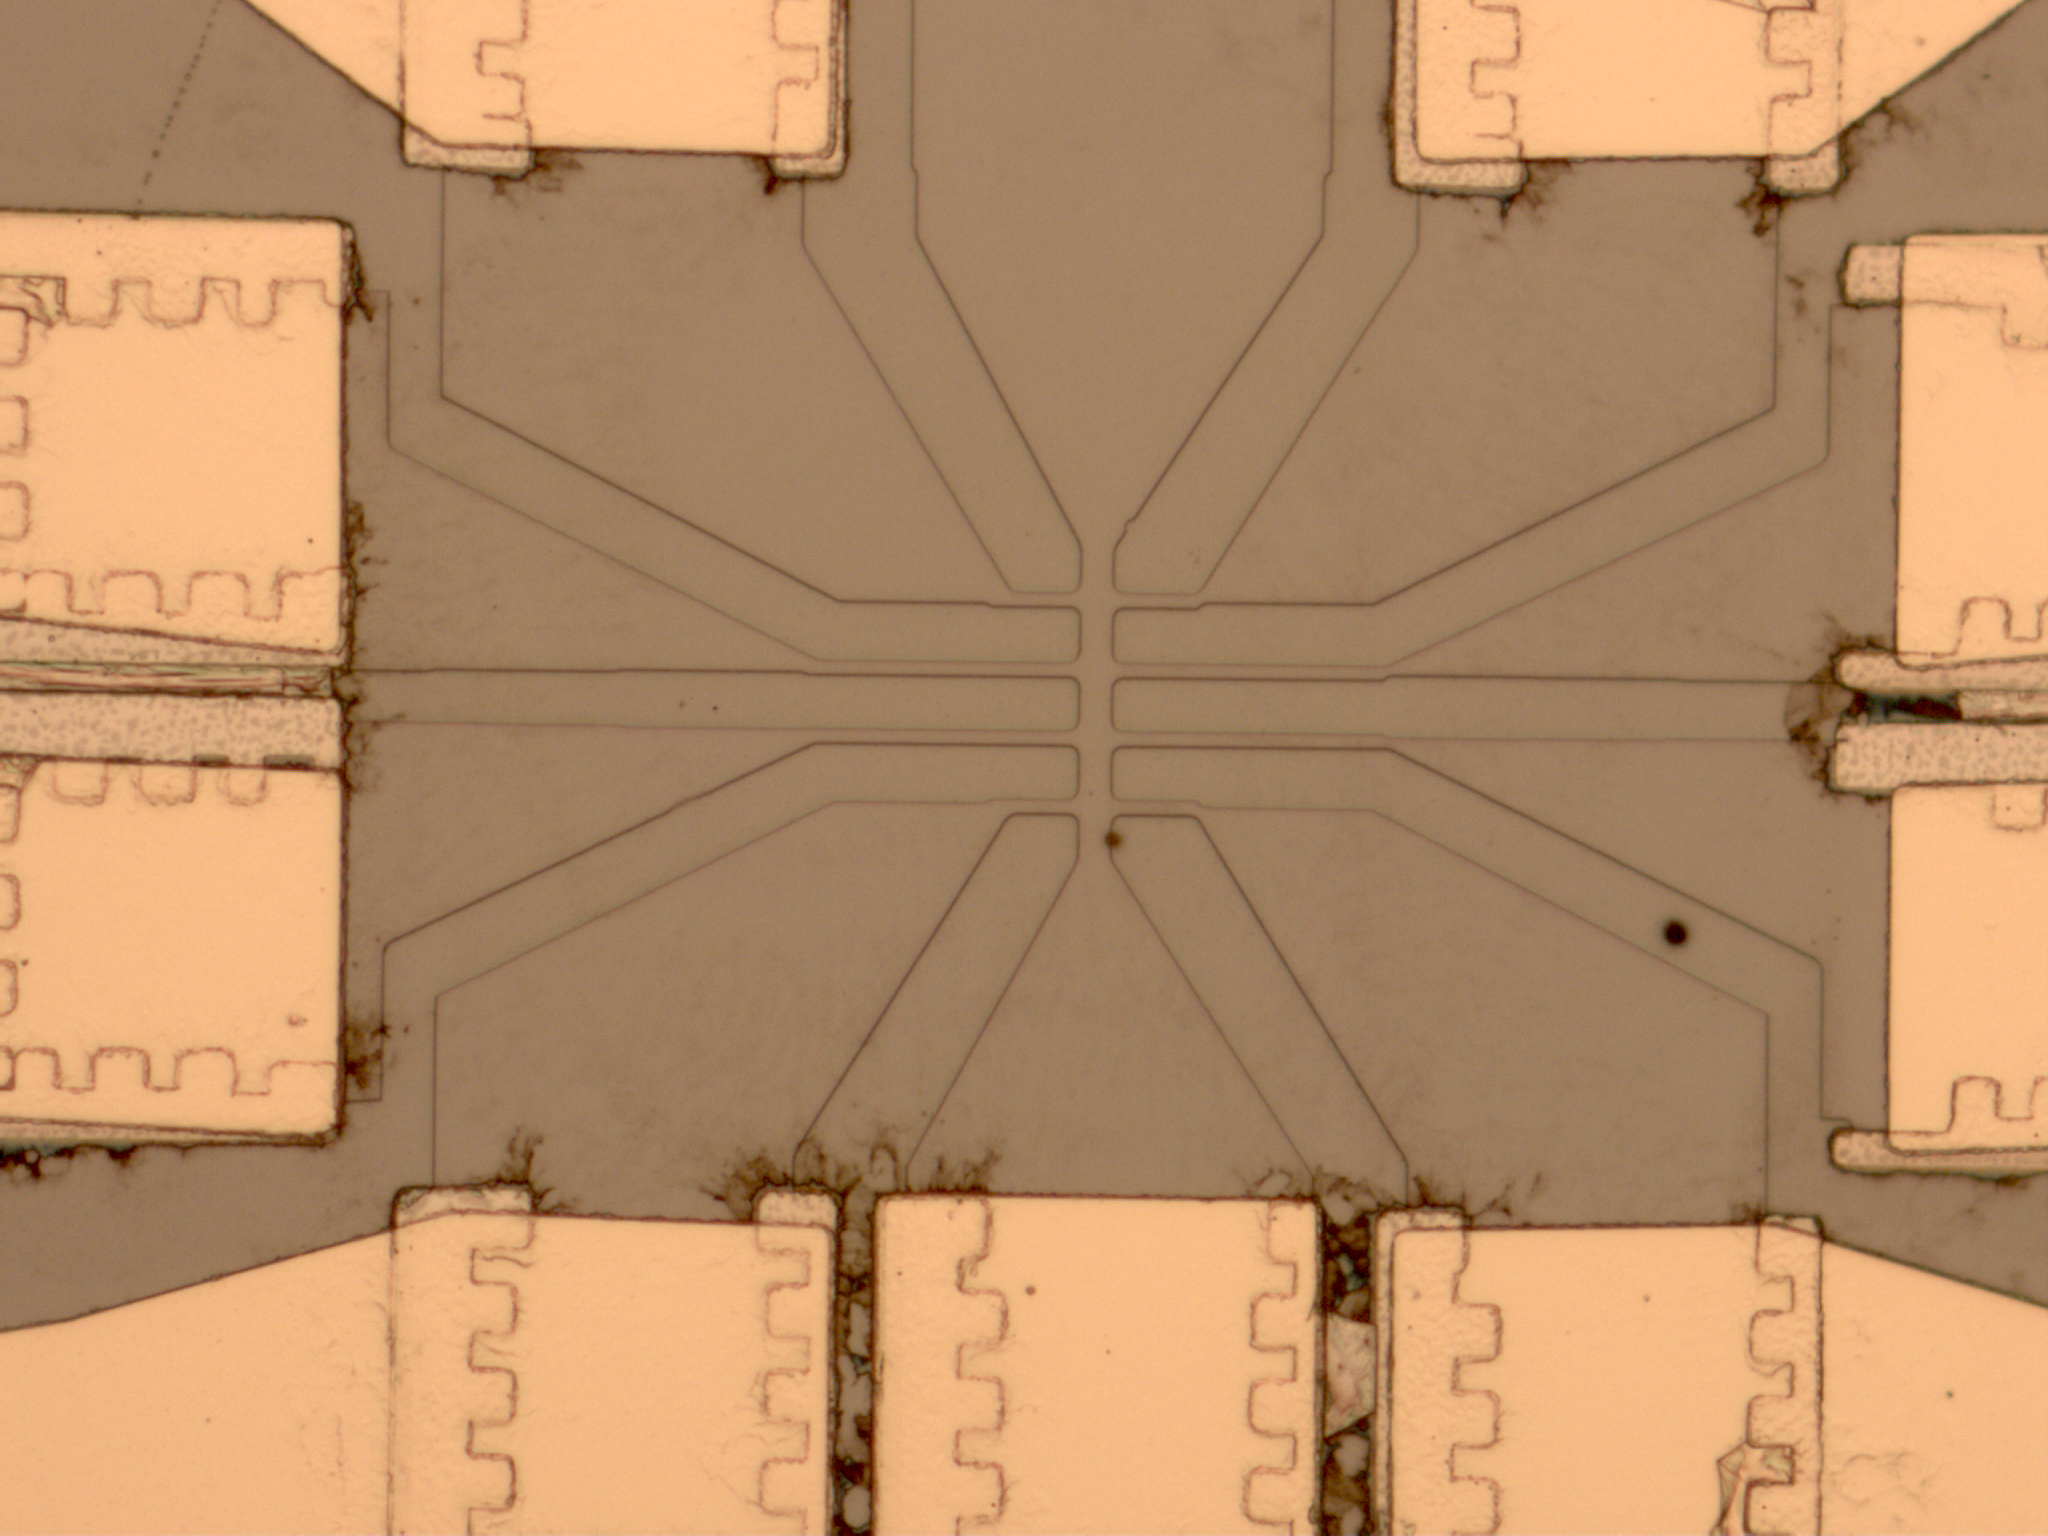
\includegraphics[width=0.5\textwidth]{4_cross_hallbar.png}
\caption{5 micron Hall crosses to be covered by bulk niobium}
\label{fig1}
\end{figure}

\begin{figure}
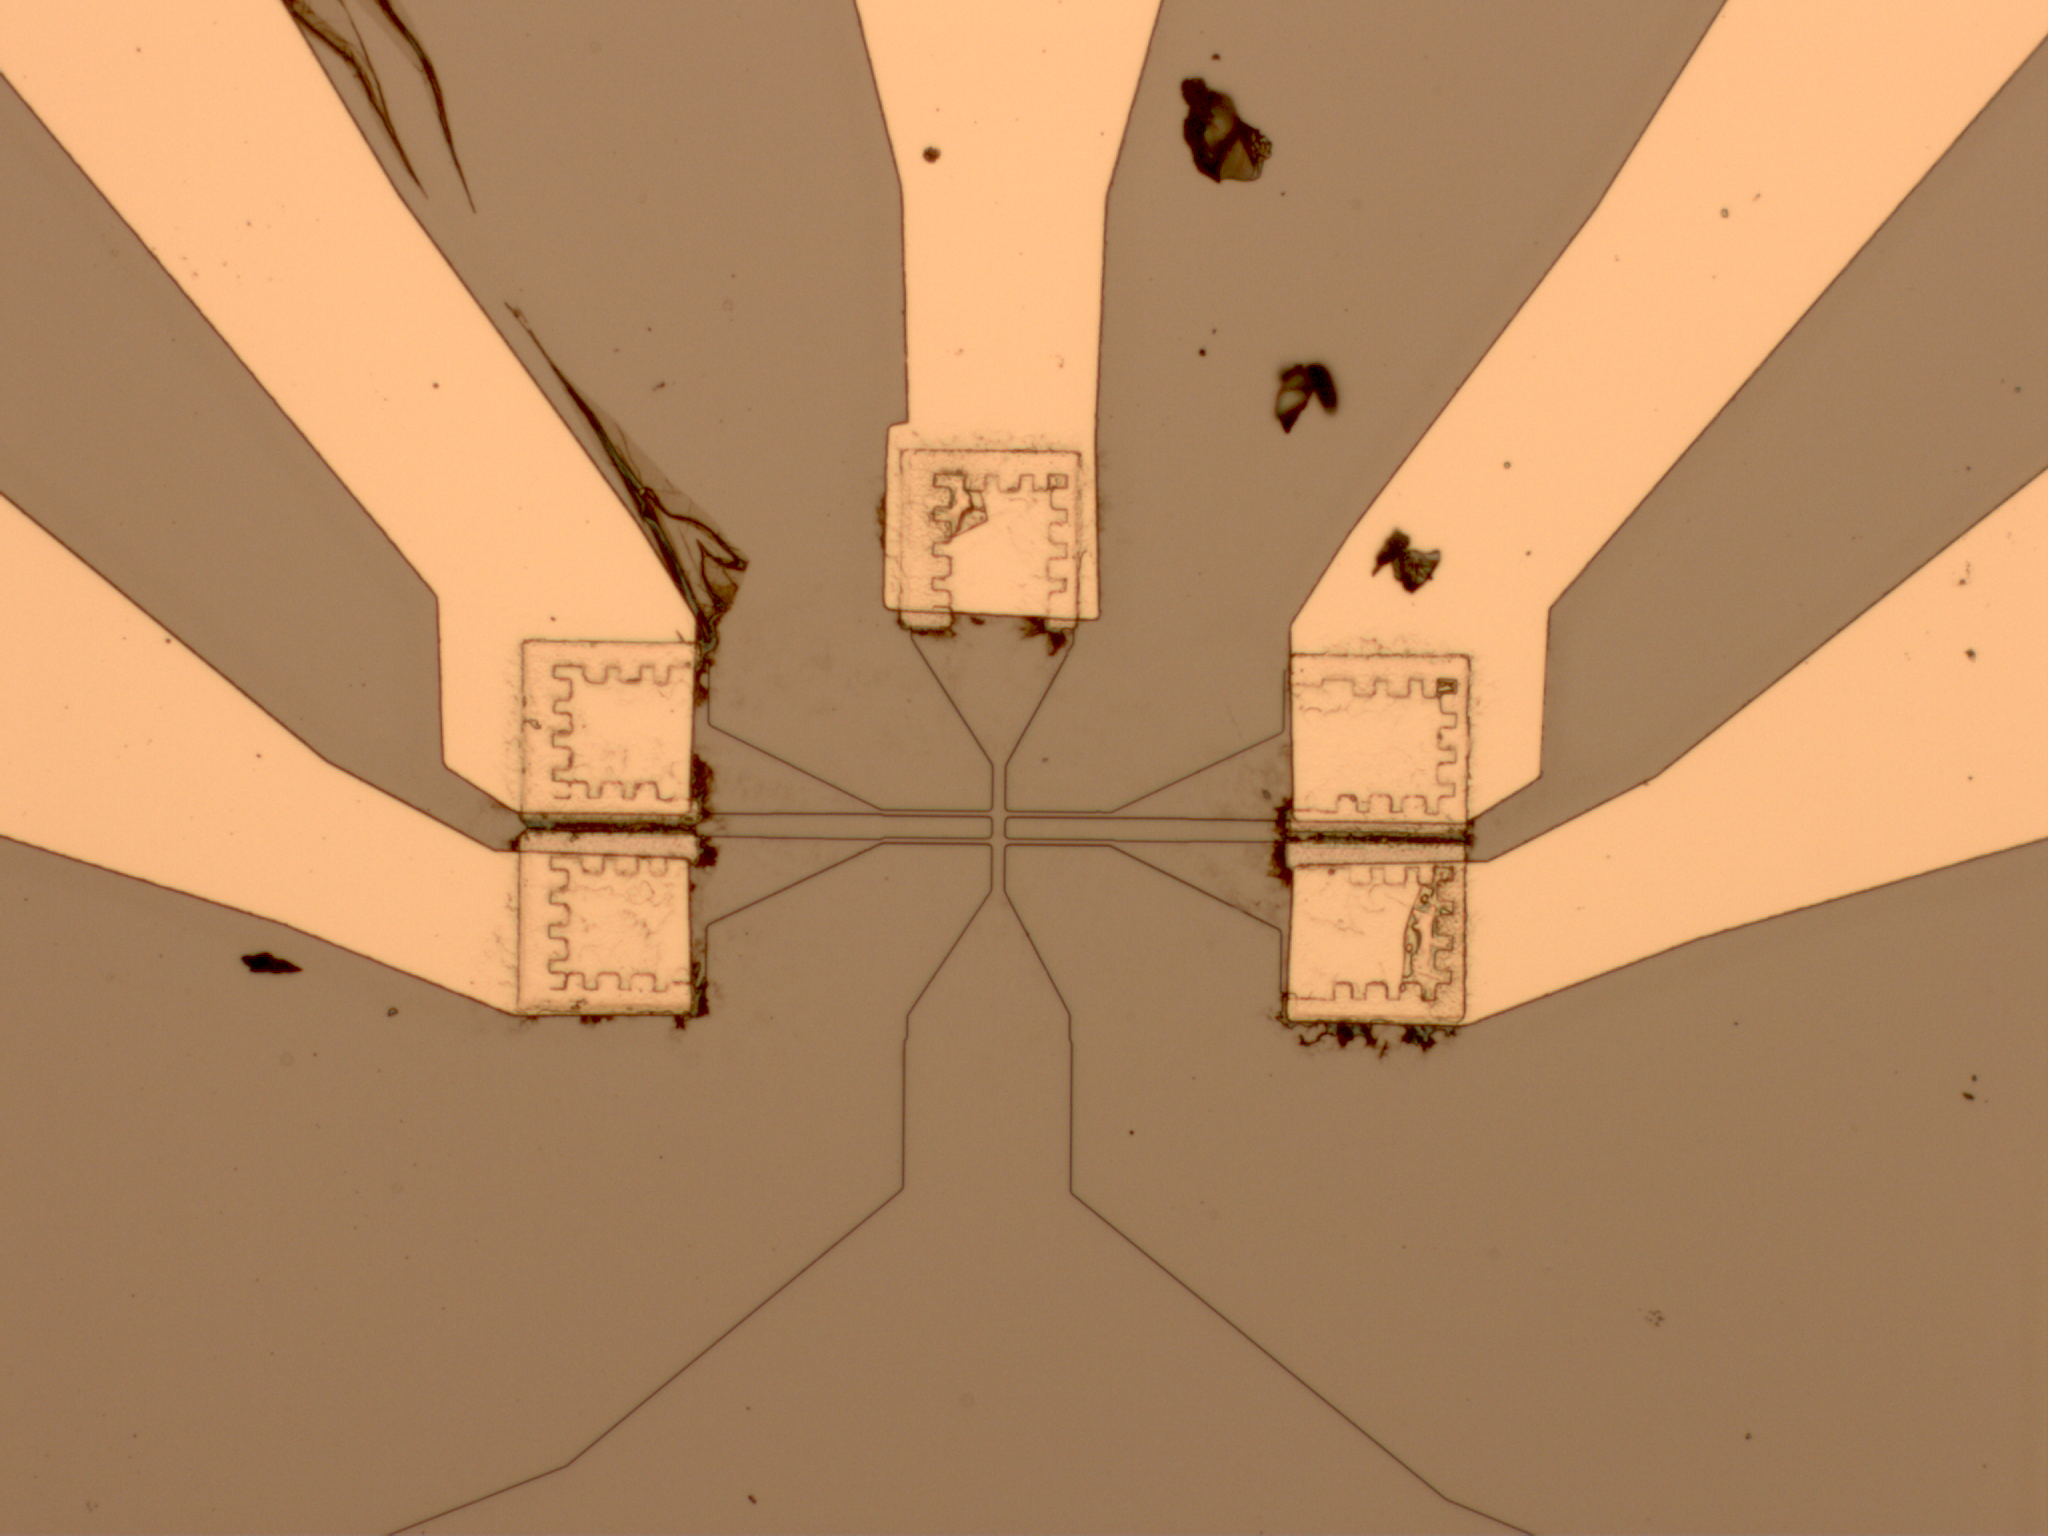
\includegraphics[width=0.5\textwidth]{2_cross_hallbar.png}
\caption{5 micron Hall crosses uncovered by the bulk niobium  }
\label{fig2}
\end{figure}
Our goal of analyzing vortex behavior in the Nioibum covered Hall crosses enforced two requirements, cryogenic temperatures and controllable magnetic field. In order to achieve these prerequisites, we used the Precision Cryogenic Systems PVS 2.5/51 LHe dewar to go down to cryogenic temperatures and a companion 6010A 1200W DC power supply to control the magnetic field in the dewar. The estimated critical temperature for bulk Niobium is 10K, so liquid helium at 4.2K served as a reasonable cryogenic medium. At this temperature, both the Niobium sample and the magnet coils are safely in their superconducting states. Our magnet produced $0.10238$T per ampere of applied current, and our current supply could produce currents up to 17A with a precision on the order of $0.01$ amps. Because we desired to achieve field strengths of $600$mT with a sensitivity of $\sim$10mT, this current supply easily handled our requirements. Further, we used a group of lock-in amplifiers to extract the Hall voltage signal at 1kHz.

In the initial setup, the niobium sample and Hall sensors were attached to a chip carrier, which were placed in a chip socket at the end of a long shaft to be lowered into the cryogenic dewar. A mount was constructed to allow finer tilt control of the chip carrier in the external magnetic field and to allow for wiring in the constricted space of the magnetic solenoid used to supply the field.

%Our original design for controlling magnetic field in the dewar involved programming the current supply to automatically produce currents corresponding with a magnetic field range. The current supply output could be set to a constant current mode, and voltage signals from a lock-in amplifier's auxiliary output controlled the magnitude of the current. The system failed to work when tested; some interaction related to inductance from the magnet and the behavior of the current supply caused the magnetic field to behave erratically. We accordingly resorted to manual manipulation of the current.

In our first attempt at data collection, complications occurred with the Hall cross devices. Once the sample was placed inside the dewar, it was imperative that we find the center of our superconducting magnet. The center of the magnet corresponds with a region of uniform magnetic field, and we designed the length of our probe to take advantage of this region. However, while the magnetic field was being controlled, there was no discernible variation in the voltage signals from the covered Hall crosses. There was a characteristic resonance at 32 Hz with a roughly $90^\circ$ phase shift, indicating a parasitic imaginary impedance. The most probable culprit for these irregularities are issues with the fabrication of the Hall cross devices. Some possible issues in the fabrication process that could explain this type of behavior include: 
\begin{enumerate}
\item The 2DEG in these samples is very thin (roughly 14 nm) and the dopants could have oxidized during an oxygen plasma and destroyed the conduction layer. 
\item The samples were deliberately over-etched in order to reduce the dimensions and it is possible that the etching procedure pinched off a segment of the conduction layer.
\item Barrier layers could have been introduced into the conduction layer via hard-baked resist as seen on the ohmic contacts in Figure \ref{fig1} and \ref{fig2}.
\item Possible scratches on the surface of the device could have damaged the conduction layer as seen in Figure \ref{fig1} and \ref{fig2}.
\item Ohmic contact might not have been achieved between the chip carrier and the chip socket 
\end{enumerate}
A combination of these factors caused the irregular behavior experienced during this phase of the experiment. 

Another issue we faced in our experimental trials involved the dimensions of our probe. Our probe barely cleared the opening of the magnet bore inside the dewar, making contact with the bore as we inserted it. When pressure is applied to the chip socket at the end of the probe, the chip releases and can be removed. On our first trial, the chip containing the Niobium and hall crosses nearly fell out of the socket, likely due to the contact with the magnet bore. We resolved this issue by attaching a cover over the end of our probe, shielding the chip socket from experiencing any mechanical force.

%\subsection{Meissner Effect Experiment}
In an effort to observe macroscopic transitions associated with the Meissner effect in Niobium despite a failed initial device, we resorted to a Hall sensor of $\sim$1mm width. This device, while insensitive to fluctuations on the order of a few vortices, still yielded interesting information about structural transitions in the vortex field between $H_{c1}$ and $H_{c2}$. To observe these transitions, two Hall crosses were used, one covered by Niobium and one uncovered to act as a control, to measure the voltage responses across the Hall cross while magnetic field was varied from a minimum strength of 0T to a maximum strength between 180 and 600mT in 10mT increments. For this sample of Niobium $H_{c1}$ is estimated to be roughly around 0T and $H_{c2}$ is estimated to be at 440mT, so this range of magnetic field is capable of containing the superconducting vortex transitions.

%\section{Results}

As expected, the uncovered Hall cross voltages responded to changes in magnetic field linearly (Fig $\ref{uplockin1}$). The covered Hall cross voltages, in contrast, exhibited more interesting behavior in response to changing magnetic field. From the plot in figure \ref{FCS}, a few main features are apparent. First, while increasing the external field from 0mT to 600mT, the measured Hall voltage on the covered cross was suppressed compared to that of the uncovered cross. After crossing $H_{c2}$, the covered and uncovered samples behaved similarly. Upon cycling down the magnetic field, the measured Hall voltage of the covered cross was higher than that of the uncovered cross, indicating flux trapping. Curiously, a hitch in the sample's tendency to trap flux seemed to occur around 100mT, at which point the measured voltage on the covered cross dropped significantly. To focus our quantitative analysis, we aim to identify $H_{c2}$ and understand the transition in flux trapping.

We distinctly detected $H_{c2}$, where our niobium sample transformed from a vortex state into a non-superconducting state, as we increased the external magnetic field strength (Fig $\ref{uplockin3}$). At magnetic fields below $H_{c2}$, we observe that the niobium suppresses the measured Hall voltage. Above $H_{c2}$, we see the destruction of the superconducting state; the linear relationship between Hall voltage and magnetic field in the covered case is practically indistinguishable from the uncovered case.

\begin{figure}
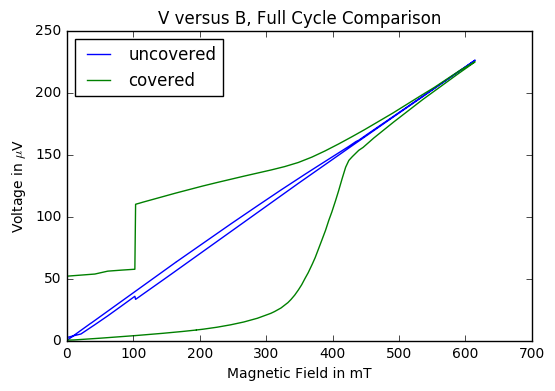
\includegraphics[width=0.5\textwidth]{FullCycleImage.png}
\caption{Covered (blue) and uncovered (green) Hall bar voltage responses shown. These measurements were done in a single magnetic field ramp up/ramp down.}
\label{FCS}
\end{figure}

We used two approaches to estimate $H_{c2}$ across our increasing field measurement runs. One approach was to use second derivate analysis, with the observation that the second derivative of the measured Hall cross voltage exhibited a strong, negative spike at the inflection seen in figure $\ref{uplockin3}$ around 420 mT. Using this method, we estimate $H_{c2}$ to be at 427(5) mT. The second method we used was to fit an exponential function to the data that was measured significantly before the inflection at $H_{c2}$, and a linear function to the data measured after $H_{c2}$. Using this method, we estimate $H_{c2}$ to be 424(9) mT. Both of these estimations are in agreement with measurements made by other groups. \cite{NbSupProp}


\begin{figure}
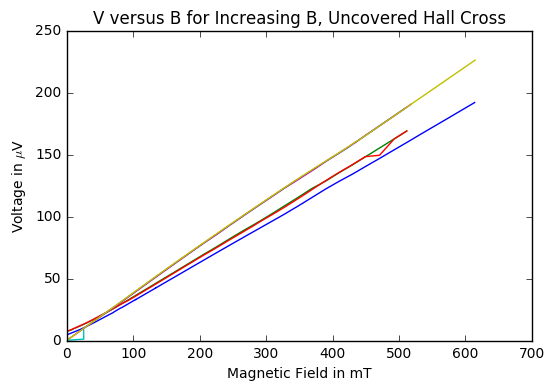
\includegraphics[width=0.5\textwidth]{UncoveredUpSweep.png}
\caption{The uncovered Hall crosses responded to changes in magnetic field linearly, as expected.}
\label{uplockin1}
\end{figure}

\begin{figure}
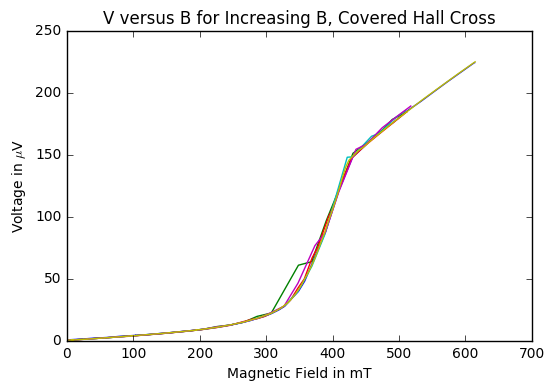
\includegraphics[width=0.5\textwidth]{CoveredUpSweep.png}
\caption{Two regimes are observable, one below $H_{c2}$ and one above $H_{c2}$. $H_{c2}$ was identified by estimating the minimum of the second derivative in the region around the transition.}
\label{uplockin3}
\end{figure}



The second interesting feature exhibited by the covered Hall cross manifested only while decreasing field. As field was reduced below $H_{c2}$, flux trapping caused the covered Hall cross to register significantly higher voltages than the uncovered cross, as predicted. Surprisingly, however, a critical value of field appeared beneath which the Hall voltage dropped by a significant fraction, as evidenced in figure \ref{DownVB}. We term this feature the flux trapping breakdown.

\begin{figure}
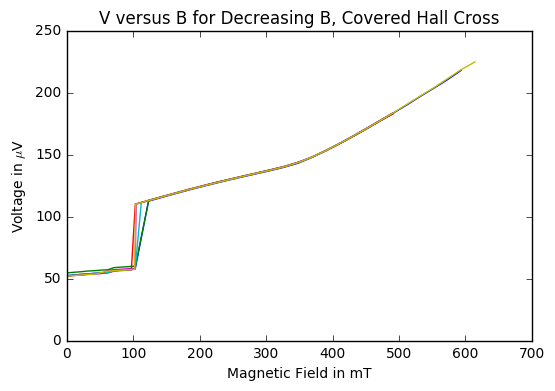
\includegraphics[width=0.5\textwidth]{DownFullVB.png}
\caption{Between $H_{c2}$ and 100mT, flux trapping is observed. However, the amount of trapped flux depreciates quickly and significantly near 100mT as long as the peak field achieved was above $H_{c2}$. We conjecture that there is a critical field strength of 100.84(14)mT corresponding to a redistribution of vortices in the superconductor.}
\label{DownVB}

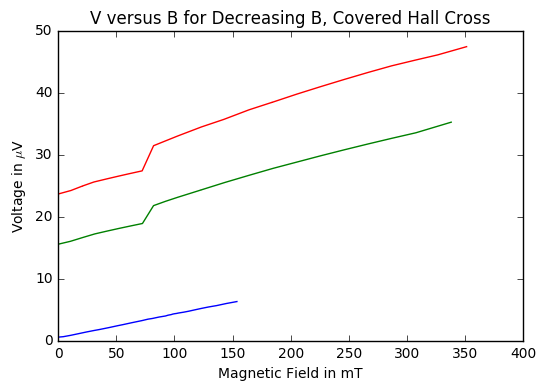
\includegraphics[width=0.5\textwidth]{DownPartVB.png}
\caption{Sweeps that did not achieve a peak field strength above $H_{c2}$ undergo the breakdown of flux trapping to a lesser extent and at a lower critical field than sweeps that did. The sweep with the lowest maximum field (150mT) did not exhibit any noticeable jump in the amount of trapped flux.}
\label{DownVB2}
\end{figure}

To understand the flux trapping breakdown, we first seek to determine where it occurs. For sweeps that had surpassed $H_{c2}$, the breakdown occurs in the same location, as depicted in figure $\ref{DownVB}$. To determine this location given our discrete data set, we assumed a uniform likelihood of the precise critical field occurring between anywhere between the last field observed before the transition and the first field observed after the transition. The uncertainty on each point was then given by the separation in field observations. The corresponding mean occurred at B$ = 100.84$mT with an uncertainty $\sigma_B = 0.14$mT. In addition to the critical field value, the amount of flux released during the transition is of interest. To measure this, we computed the ratio of voltages measured immediately before and after the transition. The mean ratio observed for sweeps that had surpassed $H_{c2}$ was 0.5213 $\pm$ .0075. Such a small fractional variation indicates that the eviction of vortices is highly systematic.

In the three sweeps that did not surpass $H_{c2}$, interesting qualitative differences surfaced, as apparent in figure $\ref{DownVB2}$. As the maximum field achieved during the sweep decreases, the flux trapping breakdown is affected in two obvious ways. One is that the critical field is reduced, and the other is that a higher percentage of the pre-transition voltage is maintained across the transition. 

To explain the behaviors witnessed solidly between our expected value of $H_{c1}$ and our observed value of $H_{c2}$, we conjecture that a routine defect in the Niobium, such as a Titanium impurity, is responsible for a frequently-occurring type of pinning site of uniform strength. Once the applied field is reduced beneath the critical breakdown field, all vortices pinned at these sites are simultaneously released, resulting in an abrupt jump in measured voltage. The relative frequency of these special pinning sites would explain the constant fractional drop in voltage for sweeps that achieved a maximum field above $H_{c2}$. Furthermore, it is possible that these pinning sites are most commonly populated at high field strengths, hence why the critical field and voltage ratio decrease when the maximum achieved field is reduced. To support or reject this hypothesis, it would be helpful to learn more about the chemical composition of the sample as well as any other potential sources of nonuniformity.

%\section{Conclusion}

We were able to measure $H_{c2}$ and the vortex eviction effect seen in a type II superconducting sample of Niobium using a Hall sensor. While increasing the external magnetic field to the sample, we measured $H_{c2}$ to be 427(5)mT and 424(9)mT, using second derivative analysis and exponential/linear fitting techniques respectively. While decreasing the external magnetic field, we estimated the vortex eviction effect to occur around $100.84(14)$mT. 

Our initial experimental goals were ambitious. We hoped to measure $H_{c1}$ and $H_{c2}$ by varying the external magnetic field through the Niobium sample and Hall sensor. After, we hoped to measure any nonuniformities in vortex density by comparing measurements from several small Hall crosses located throughout the sample. Finally, we hoped to apply a current to the superconductor and observe the responses of the spatial density of vortices and their velocity disribution across the sample. Due to complications in fabrication and our experimental setup, we were unable to pursue this line of experimental reasoning. However, we were still able to measure $H_{c2}$ and quantify vortex eviction effects during our magnetic field decrease phase for our obtained sample of Niobium. In the future, it would be interesting to explore the possibilities of vortex behavior analysis with smaller and more sensitive Hall sensors.

We would like to thank David Goldhaber-Gordon, Stephen Kuenstner, John Bartel, and Rick Pam for their help with our planning and execution of this experiment.

\begin{thebibliography}{9}
% APA

\bibitem{SQUID}
  B. Plourde, D. V. Harlingen, R. Besseling, M. Hesselberth, and P. Kes, Physica C: Superconductivity 341-348, 1023 (2000).
  % \textit{Vortex dynamics in thin superconducting strips observed by Scanning SQUID Microscopy}, http://dvh.physics.illinois.edu/publications/Vortex%20stuff%20with%20Britton.pdf

\bibitem{CFNIOBIUM_1}
   Saito, K., and Tsukuba-shi, O. (2001). Critical field limitation of the niobium superconducting RF cavity.
\begin{comment}
"The sample is a 2.5mm
thick and 5 mm wide and 150 mm long (rectangle crosssection)"..much larger sample Niobium, getting HC_1 and HC_2 (around 4K) of .140 and .300 T respectively. Should possibly look into the fabrication for the sample we got data from.

https://accelconf.web.cern.ch/accelconf/srf01/papers/ph003.pdf
\end{comment}
 
\bibitem{VortexMotion_1}
	Lefebvre, J. (2004). Peak Effect, Hall Effect and Vortex Phases in FexNi1-xZr2 Superconducting Glasses (Doctoral dissertation, McGill University).	

\bibitem{VortexInteraction_1}
	Xu, X. B., Fangohr, H., Ding, S. Y., Zhou, F., Xu, X. N., Wang, Z. H., ... and Dou, S. X. (2011). Phase diagram of vortex matter of type-II superconductors. Physical Review B, 83(1), 014501.
\begin{comment}
Long range and short range interaction mentioned...pretty interesting, "Langevin
molecular-dynamical simulation". 

https://journals.aps.org/prb/pdf/10.1103/PhysRevB.83.014501
\end{comment}

\bibitem{NbSupProp}
	Stromberg, Thorsten Fredrick, "The superconducting properties of high purity niobium " (1965). \textit{Retrospective Theses and Dissertations}.
Paper 3283.
\begin{comment}
Paper on superconducting bulk niobium to cite value for Hc1 and Hc2
\end{comment}
\end{thebibliography}


\end{document}
